%\documentclass[9pt]{article}
\documentclass[article]{IEEEtran}
\usepackage{graphicx}
\usepackage{float}
\usepackage{amsmath}
\usepackage{amsfonts}
\usepackage[brazilian]{babel}
\usepackage[utf8]{inputenc}
\usepackage[backend=biber]{biblatex}
\usepackage{csquotes}
\usepackage{gensymb}
%\usepackage{docmute}
\usepackage{array}
\usepackage{multicol}
\usepackage{geometry}
\usepackage[T1]{fontenc}
\addbibresource{rel_parcial_erik_perillo_2sem2016.bib}

\newcommand{\fromeng}[1]{\footnote{do inglês: \textit{#1}}}
\newcommand{\tit}[1]{\textit{#1}}
\newcommand{\tbf}[1]{\textbf{#1}}
\newcommand{\ttt}[1]{\texttt{#1}}
\newcommand{\ie}{i.~e.~}
\newcommand{\eg}{e.~g.~}

\begin{document}

\newgeometry{margin=1.0in}

\begin{titlepage}
	\centering
	{\scshape\Large Relatório Parcial\par}
	\vspace{1.5cm}
	{\huge\bfseries Atenção visual para sistemas robóticos com Deep Learning\par}
	\vspace{1cm}
	{\itshape Aluno: Erik de Godoy Perillo\par}
	{\itshape Orientadora: Profa. Dra. Esther Luna Colombini\par}
	\vspace{0.5cm}
	\vfill
    Instituto de Computação\\
	Universidade Estadual de Campinas
	\vfill
	{\large \today\par}
\end{titlepage}

\newpage

%\begin{multicols}{2}
\section{Introdução}
A capacidade de percepção e construção de um modelo da realidade ao seu redor
é fundamental para que sistemas robóticos interajam com o ambiente e executem
tarefas diversas e complexas que podem ter as mais variadas utilidades para
os humanos.
Um componente fundamental para isso é a habilidade de dar foco apenas ao
relevante, evitando assim o processamento desnecessário de enormes quantias
de dados.

A atenção é um processo que faz parte do dia a dia de diversos seres vivos
em diversas maneiras e é razoável inspirar-se nela para a construção de
mecanismos semelhantes para a construção de sistemas de inteligência
artificial em máquinas.
Tal área tem sido foco de estudo há anos, resultando em diversas teorias
em psicologia sobre a atenção humana que inspiraram a implementação de
modelos computacionais bem sucedidos, que geram imagens semelhantes ao
exemplo da figura~\ref{fig:example}.

Em trabalhos anteriores, foi desenvolvido um modelo de saliência
visual com uma rede neural convolucional eficiente~\cite{oldic}.
A arquitetura da rede permitiu que fossem atingidos resultados comparáveis
ao estado da arte, com um número de parâmetros reduzido em 75\%.
Neste trabalho, objetivamos construir um modelo de saliência visual eficiente
para vídeo.

\begin{center}
\begin{figure}[t]
\begin{tabular} {cc}
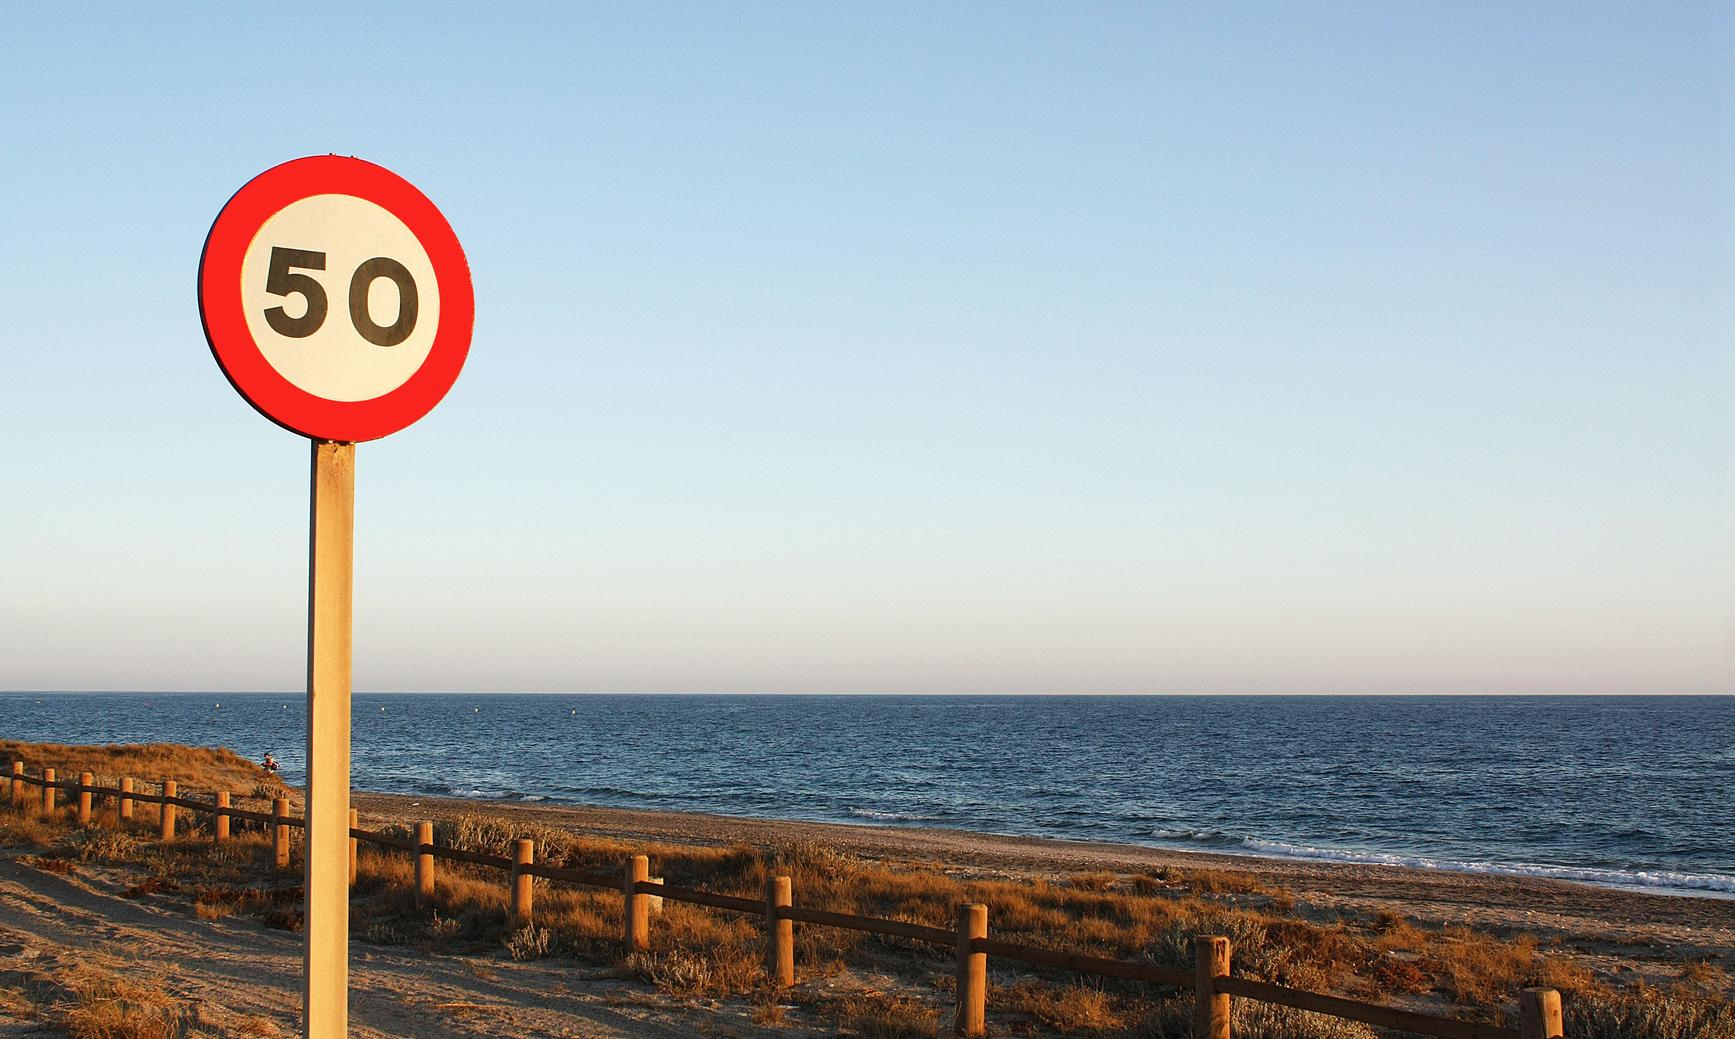
\includegraphics[width=0.22\textwidth]{./img/traffic_sign_s.jpg} &
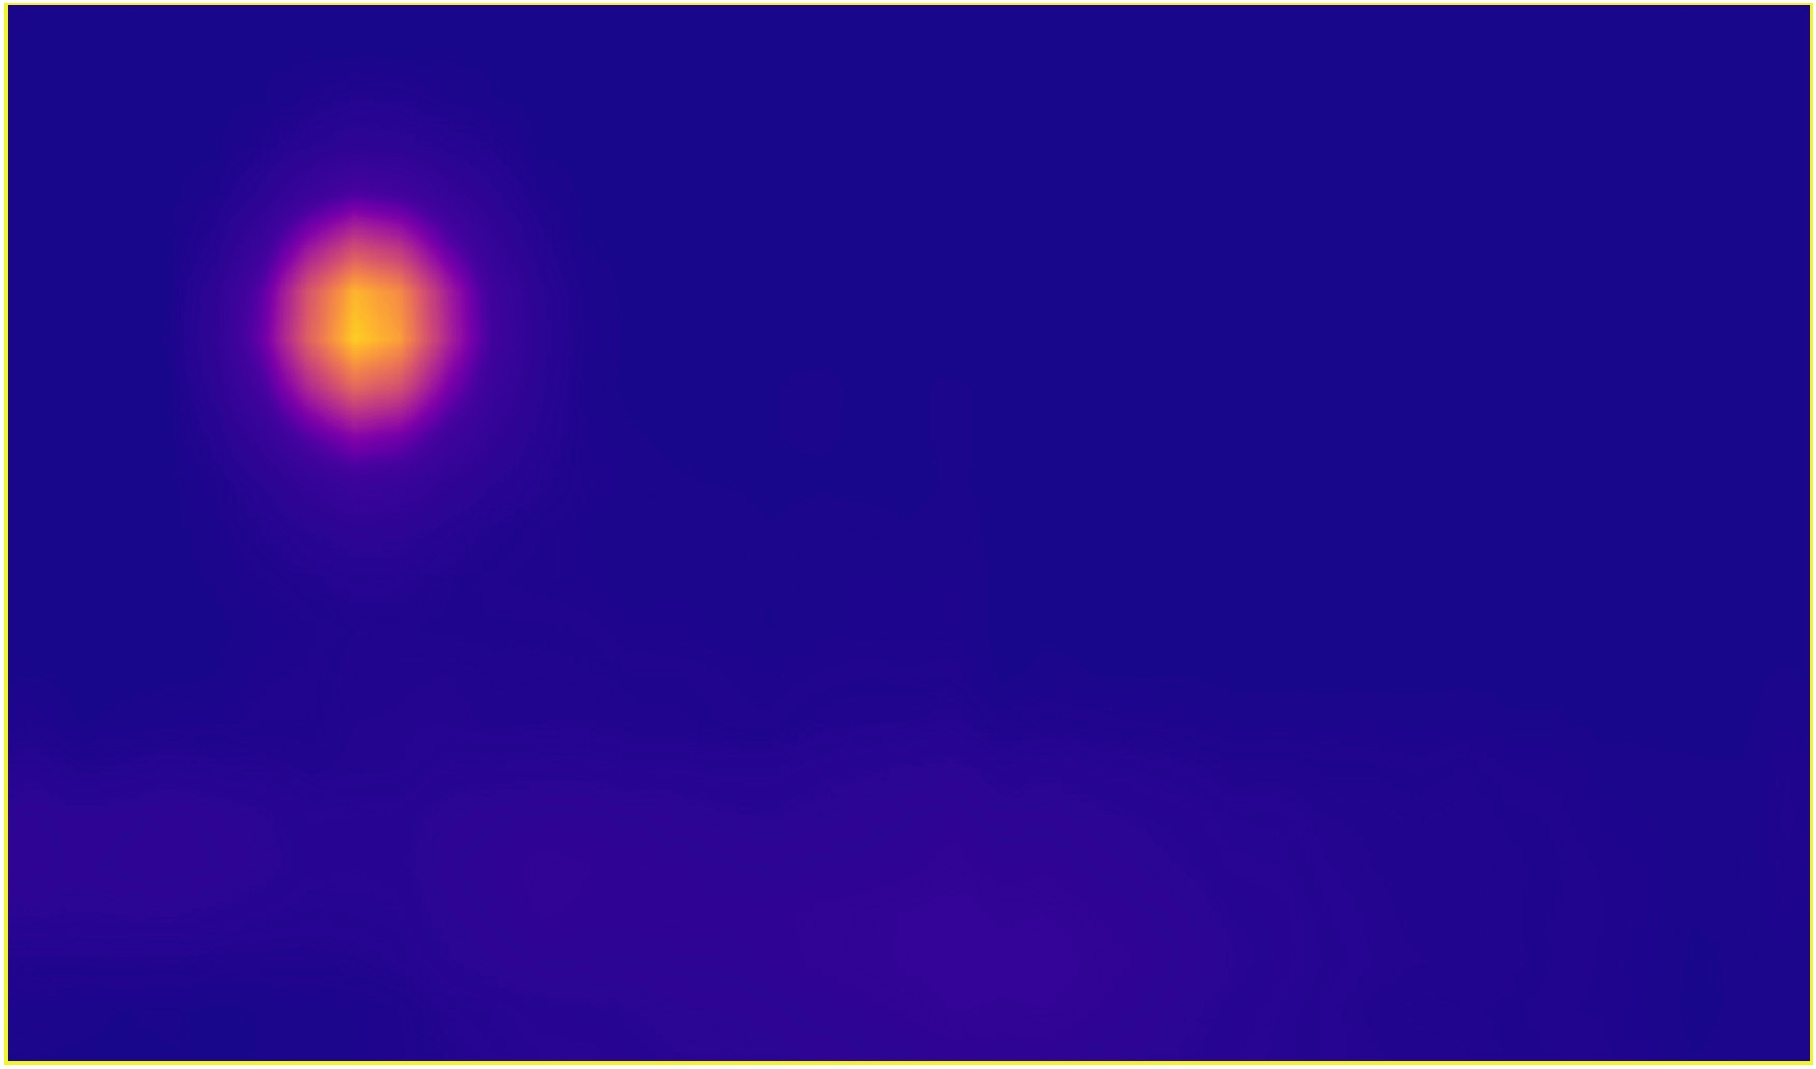
\includegraphics[width=0.22\textwidth]{./img/traffic_sign_m.jpg}\\
(a) & (b)
\end{tabular}
\caption{Examplo de saliência visual.
    b) é o mapa de saliência onde regiões mais brilhantes (cores mais quentes)
    representam regiões mais salientes para humanos na imagem original a).}
\label{fig:example}
\end{figure}
\end{center}

\subsection{Objetivos da primeira parte do projeto}
Os objetivos principais para o primeiro semestre do trabalho eram:
\begin{itemize}
    \item Revisão bibliográfica sobre atuais trabalhos em vídeo.
    \item Escolha das técnicas mais adequadas para o processo atencional
        e adaptação do das técnicas conhecidas para vídeo.
    \item Implementação de um modelo atencional para vídeo.
\end{itemize}
Embora haja relevantes avanços recentes na detecção de saliência visual para
imagens estáticas, não há ainda na literatura um considerável número de
trabalhos focando em vídeo.
Ainda assim, com estudo da literatura já existente em atenção e no número
reduzido de trabalhos que focam em vídeo, houve progresso.

\section{Resumo das atividades}
\subsection{Revisão Bibliográfica}
Um conceito importante para o entendimento da literatura do meio é o de
\tit{Bottom-up vs. Top-down}: Por componente \tit{bottom-up} de
atenção entende-se saliências instintivas percebidas por mudanças
e/ou contrastes muito grandes em uma cena. O componente \tit{top-down}
é aquele que dá saliência variável às \tit{features} de acordo
com a meta do agente do momento.
A maioria dos modelos computacionais baseia-se em teorias formadas na
psicologia.
Duas das mais famosas são a \tit{Feature Integration Theory}
(FIT)~\cite{TreismanGelade1980} e a
\tit{Guided Search}~\cite{Wolfe1989}.
Ambas provêm contribuições importantes para o entendimento dos processos
de saliência visual.

Para saliência visual estática (única imagem),
relevantes avanços foram feitos nos últimos anos com o uso de
\tit{Deep Learning}.
Modelos como \tit{DeepFix}~\cite{deepfix}, \tit{SALICON}~\cite{salicon} e
\tit{MLNet}~\cite{mlnet} usam arquiteturas de redes neurais completamente
convulucionais. Muitos modelos atuais usam redes pré-treinadas como a
VGG-16 com uma etapa de refinamento.
Tais modelos são o estado da arte atual para imagens estáticas.

Saliência estática, entretanto, não é suficiente.
Em humanos, há um importante fenômeno: IOR
(do inglês: \tit{Inhibition of Return}.)
Tal efeito faz com que o foco atencional mude com o passar do tempo.
Isso provê uma vantagem evolutiva pois permite ao ser explorar o ambiente ao
seu redor.
Assim, uma região de uma imagem que um modelo estático identificou como
altamente saliente pode não o ser dependendo do contexto da sequência
de imagens e de focos atencionais (figura~\ref{fig:ior}).

\begin{center}
\begin{figure}[t]
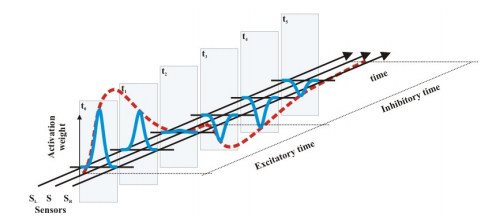
\includegraphics[width=0.5\textwidth]{./img/ior.png}
\caption{Exemplo de variação de estímulo atencional no tempo com IOR.}
\label{fig:ior}
\end{figure}
\end{center}

O principal trabalho estudado que aborda a saliência para vídeo~\cite{vidfix},
onde um modelo com uma rede neural convolucional \tit{end-to-end}
é usada para a geração de mapas de saliência visual.
Sua arquitetura combina uma rede convolucional treinada para imagens estáticas
a uma nova rede convolucional para sequências de frames de vídeos.
Tal modelo obtém resultados melhores que apenas a rede para imagens estáticas
no dataset DAVIS~\cite{davis}.

A revisão bibliográfica feita mostrou-se fundamental para os trabalhos
desenvolvidos no semestre.

\subsection{Modelo atencional}
\subsubsection{Modelo estático}
O primeiro modelo desenvolvido em trabalhos anteriores \tit{DeepPeek},
obteve métricas consistentemente entre os dez primeiros colocados no
\tit{MIT Saliency Benchmark}~\cite{mitsal}.
Sua arquitetura se destaca por ser uma rede neural totalmente convolucional
feita especificamente para a detecção de saliência visual e treinada
do zero, com $3717841$ parâmetros.
Sua entrada consiste em imagens no espaço de cor LAB, mais semelhante ao
sistema visual humano.

A primeira contribuição deste trabalho foi uma versão melhorada do
modelo antigo para imagens estáticas (figura~\ref{fig:unet}):
com menos parâmetros ($2323145$) e mesmo desempenho, a arquitetura é baseada na
\tit{Unet}~\cite{unet}, e é mais flexível para futuras alterações que adaptem
o modelo para vídeo.
O novo modelo também usa imagens em LAB e foi treinado usando-se os
\tit{datasets SALICON}~\cite{salicon} e \tit{Judd}~\cite{judd}.

\begin{center}
\begin{figure}[t]
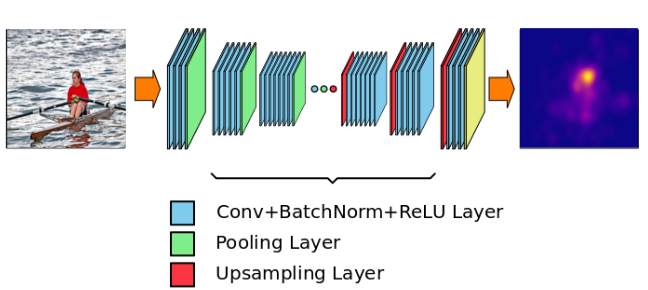
\includegraphics[width=0.5\textwidth]{./img/unet.png}
\caption{Arquitetura do modelo proposto para imagens estáticas.}
\label{fig:unet}
\end{figure}
\end{center}

\begin{table}
\centering
	\small
\label{table:unet}
\caption{Número de filtros em cada camada da rede proposta.}
\begin{tabular}{|c|c|c|}
	\hline
    Bloco & Tipo & Número de filtros\\
    \hline
    & conv & 32\\
    input/downsample & conv & 32\\
    & conv & 32\\
    \hline
    & conv & 48\\
    downsample & conv & 48\\
    & conv & 48\\
    \hline
    & conv & 64\\
    downsample & conv & 64\\
    & conv & 64\\
    \hline
    & conv & 96\\
    downsample & conv & 96\\
    & conv & 96\\
    \hline
    & conv & 128\\
    downsample & conv & 128\\
    & conv & 128\\
    \hline
    & conv & 180\\
    upsample & conv & 180\\
    & conv & 180\\
    \hline
    & conv & 128\\
    upsample & conv & 128\\
    & upconv & 128\\
    \hline
    & conv & 96\\
    upsample & conv & 96\\
    & upconv & 96\\
    \hline
    & conv & 64\\
    upsample & conv & 64\\
    & upconv & 64\\
    \hline
    & conv & 48\\
    upsample/output & conv & 48\\
    & upconv & 48\\
    \hline
\end{tabular}
\end{table}

\subsubsection{Implementação de IOR}
O principal objetivo de uma implementação de \tit{IOR} para mapas de
saliência contínuos é simular o curso atencional em humanos.
Isso é feito aumentando-se a probabilidade de áreas com menos foco atencional
no passado de serem atendidas no futuro e, de modo análogo, diminuindo-se
a probabilidade de áreas com grande saliência de serem altamente avaliadas
em um período de tempo próximo.
Para isso, dado um fluxo de imagens $F$, com $S_t$ a saliência de um
ponto $(x, y)$
no mapa no momento $t$, computa-se o mapa de inibição de retorno $IOR_{t+1}$ da
seguinte forma:
$$IOR_{t+1} = \frac{k_pP(t) + k_iI(t) + k_dD(t) + k_cC}
{k_p + k_i + k_d + k_c}$$
com
$$P(t) = 1 - S_t$$
$$I(t) = \frac{1}{1 + \int_{0}^{t} S_\tau d\tau}$$
$$D(t) = (1 + S'(x)|_{x=t})/2$$
$C$ sendo o mapa constante.

$P(t)$ diz respeito à parte proporcional, o mapa de saliência
no momento imediato antes do novo mapa.
$I(t)$ diz respeito à parte integrativa, isto é, o quanto esta área foi
saliente no passado.
Quanto mais saliente uma região já foi, maior é sua inibição.
$D(t)$ diz respeito à parte derivativa. Se a saliência mudou rapidamente,
esta área merece um realce.
$C$ é o mapa constante. Todos os mapas variam no intervalo $[0, 1]$.
$k_p, k_i, k_d, k_c$ são constantes que controlam a influência de
cada componente no mapa final.
Com base nos experimentos realizados, os melhores valores para
$k_p, k_i, k_d, k_c$ são, respectivamente, $0.2, 0.4, 0.1, 0.3$.
Figura~\ref{fig:iorvid} ilustra um exemplo de mapa de IOR gerado com a técnica.

\begin{center}
\begin{figure}[t]
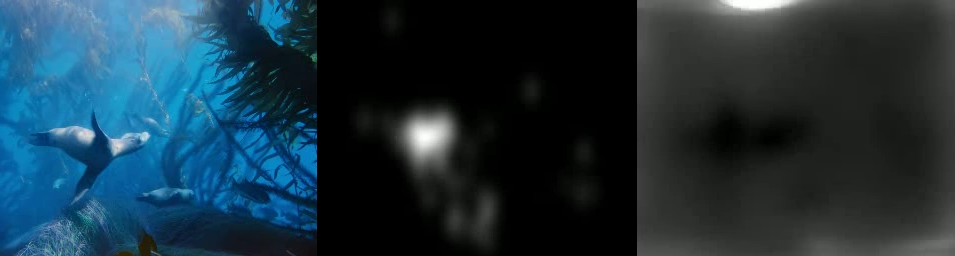
\includegraphics[width=0.5\textwidth]{./img/iorvid.png}
\caption{Exemplo de geração de mapa de IOR.
    À esquerda, um frame do vídeo.
    No centro, o mapa de saliência correspondente ao frame.
    À direita, o mapa de IOR, com valores mais escuros onde há maior inibição.}
\label{fig:iorvid}
\end{figure}
\end{center}

\subsubsection{Modelo final}
O modelo final combina a saída da rede estática com IOR.
Dado $R_{t+1}$, o valor da saliência calculado pelo método estático,
o mapa final $S_{t+1}$ é dado por:
$$S_{t+1} = R_{t+1}*IOR_{t+1}$$

\subsubsection{Implementação}
Todas as etapas do modelo descritas aqui foram implementadas.
A linguagem utilizada foi \tit{Python}, usando-se \tit{OpenCV}, \tit{numpy}
e \tit{tensorflow}.
O código está disponível de modo público em \ttt{https://github.com/erikperillo/att}.

\subsection{Avaliação de desempenho}
Foi feita uma pesquisa das métricas e \tit{datasets} mais usados para
avaliação dos modelos computacionais, pois isso
é muito importante para o avanço do trabalho.

\subsubsection{\tit{SAVAM}}
SAVAM é um dataset com 41 vídeos com informação de mapas contínuos de
saliência obtida por dados de \tit{eye-tracking} de observadores~\cite{savam}.
Por conter vídeos de variados contextos, o dataset foi considerado a
mais completa das opções e então utilizado para avaliação do desempenho.

\subsubsection{Métricas}
Muitas das métricas aqui mostradas são discutidas em~\cite{judd2},
onde a aplicabilidade, significado, vantagens e desvantagens
de cada uma são discutidas mais a fundo. Aqui daremos apenas uma breve
descrição das mesmas.

\begin{itemize}
	\item \ttt{Similarity}\newline
	Definido como:
	$$SIM(P, Q) = \frac{1}{N}\sum\limits_{i=1}^N{min(P_i, Q_i)}$$
	Com $P$ e $Q$ indo de $0$ a $1$. Um valor de $1$ define mapas idênticos
	e $0$ mapas totalmente diferentes.
	Ambos os mapas são normalizados pela soma de cada um.
	Usado em~\cite{mit-300}.

	\item \ttt{Correlation Coefficient}\newline
	\ttt{Similarity} penaliza \tit{false negatives} mais que
	\tit{false positives}~\cite{judd2}. A métrica \ttt{CC} trata os dois
	simetricamente. Dada por:
	$$CC(P, Q) = \frac{cov(P,Q)}{\sigma(P)\sigma(Q)}$$
	Onde $P$ é normalizado no intervalo $[0, 1]$.
	Usado em~\cite{mit-300}.

	\item \ttt{Mean-square error}\newline
	Dado por:
    $$MSE(P, Q) = \frac{1}{N}\sum\limits_{i=1}^N{{(P_i - Q_i)}^2}$$
	Usado em~\cite{mit-300}.
\end{itemize}

\subsection{Resultados}
Usando-se apenas o modelo para saliência estática, obteve-se um resultado
pior do que quando o ajuste para IOR foi feito.
A tabela~\ref{table:results} ilustra os resultados.

\begin{table}
\centering
	\small
\label{table:results}
\caption{Resultados do modelo estático e com IOR.}
\begin{tabular}{|c|c|c|}
	\hline
    Modelo & Métrica & Valor médio\\
    \hline
    Estático & CC & 0.41\\
    \hline
    Estático & SIM & 0.37\\
    \hline
    Estático & MSE & 0.40\\
    \hline
    Estático + IOR & CC & 0.46\\
    \hline
    Estático + IOR & SIM & 0.41\\
    \hline
    Estático + IOR & MSE & 0.11\\
    \hline
\end{tabular}
\end{table}

\subsection{Conclusão}
Neste trabalho, obteve-se um modelo de rede neural convolucional para
imagens estáticas eficiente para detecção de saliência visual.
Combinado a um método de simulação do fenômeno de \tit{Inhibition of Return},
o modelo obteve resultados melhores para detecção de saliência visual
em vídeos.

\section{Próximos passos}
O próximo passo é a concepção de um sistema que usa aprendizado de máquina
de uma maneira \tit{end-to-end}, sem a necessidade de entrada manual de
IOR.

\printbibliography

%\end{multicols}
\end{document}
